FlexPMS er opbygget af adskillige tråde, som alle kan snakke sammen ved at sende beskeder til hinanden. Trådene håndterer udelukkende beskeder sendt til dem udefra, og står derfor udelukkende i blokerende kald til en besked-kø (et \textit{MessageQueue}-objekt) så længe de ikke er ved at håndtere en indkommende besked. Trådene nedarver fra \textit{MessageThread} og har pointers til de tråde, som de skal kunne sende beskeder til.

\KlasseDiagram{1}{FlexPMS}{EventSystem}


\subsubsection{MessageThread}
Klassen, som er en specialisering af \textit{Thread}, stiller funktionalitet til rådighed til at indgå i det event-baserede beskedsystem. Ved at nedarve fra \textit{MessageThread} bliver en klasse til en modtager af beskeder, og kan i den forbindelse nøjes med at implementere en \textKode{dispatch()} metode, som kaldes hver gang tråden modtager en besked via dens \textKode{send()} metode. \textKode{dispatch()} modtager to argumenter; et event-ID samt en pointer til et \textit{Message}-objekt, der evt. kan være \textKode{NULL}. Dispatch bør overholde reglen om, at kalde en funktion til at håndtere beskeden alt efter hvilket event-ID den modtager, hvilket typisk implementeres vha. en switch-case.\\\\

\textKode{send()} tager ligeledes to argumenter; et event-ID samt en pointer til et \textit{Message}-objekt. Det er afsenderen, som skal allokere \textit{Message}-objektet, men \textit{MessageThread} sørger selv for, at de-allokere det efter \textKode{dispatch()} er kaldt hos modtageren, og beskeden er håndteret.\\\\

Nedenfor ses et eksempel på kommunikation mellem to tråde, \textit{MessageThread1} og \textit{MessageThread2}, initieret af \textit{MessageThread1}, hvor \textit{MessageThread2} svarer på beskeden. 

\SekvensDiagram{1}{FlexPMS}{MessageThread}

\textit{MessageThread} laver udelukkende blokerende kald til dens besked-kø (et \textit{MessageQueue}-objekt), og dermed undgår vi at stå og bruge CPU-tid i løkker, som ikke udfører noget. Det betyder, at alle klasse som nedarver fra \textit{MessageThread} udelukkende håndterer events sendt til dem udefra. På den måde lægges tråde til at sove så længe der ikke er noget at lave, og programmet vil bruge minimalt CPU-tid.


\StateDiagram{0.5}{FlexPMS}{MessageThread}

\subsubsection{Arkitekturspecifikke metoder}

\funk{virtual void init()}{Abstrakt metode, som kaldes inden der begyndes at hente beskeder fra beskedkøen. Kan bruges til at lave initiering af objektet. Metoden kan overskrives af klasser, som nedarver fra \textit{MessageThread}}{Ingenting}
{}

\funk{void send(unsigned long id, Message* msg = NULL)}{Sender en besked til tråden, ved at lægge en besked i dens beskedkø}{Ingenting}
{
\funkArg{id}{Et ID, som beskriver det event der sendes}
\funkArg{msg}{En pointer til et \textit{Message}-objekt, som kan holde på yderligere data}
}

\funk{virtual void dispatch(unsigned long event\_id, Message* msg))}{Abstrakt metode, som kaldes hver gang tråden modtager en besked. Metoden skal overskrives af klasser, som nedarver fra \textit{MessageThread} til at håndtere indkommende beskeder}{Ingenting}
{
\funkArg{event\_id}{Et ID, som beskriver det event der sendes}
\funkArg{msg}{En pointer til et \textit{Message}-objekt, som kan holde på yderligere data. Kan være \textKode{NULL}}
}


\subsubsection{MessageQueue}

Klassen er en FIFO kø, som er trådsikret, dvs. sikret mod de problemer der kan opstå i forbindelse med at tilgå den parallelt fra forskellige tråde. \textit{MessageQueue} er implementeret via en queue (fra STL) og benytter sig at pthread’s \textit{mutex} og \textit{conditional variable} til at synkronisere mellem tråde. \textit{MessageQueue} er udelukkende brugt internt i \textit{MessageThread}.

\begin{figure}[H]
	\centering
	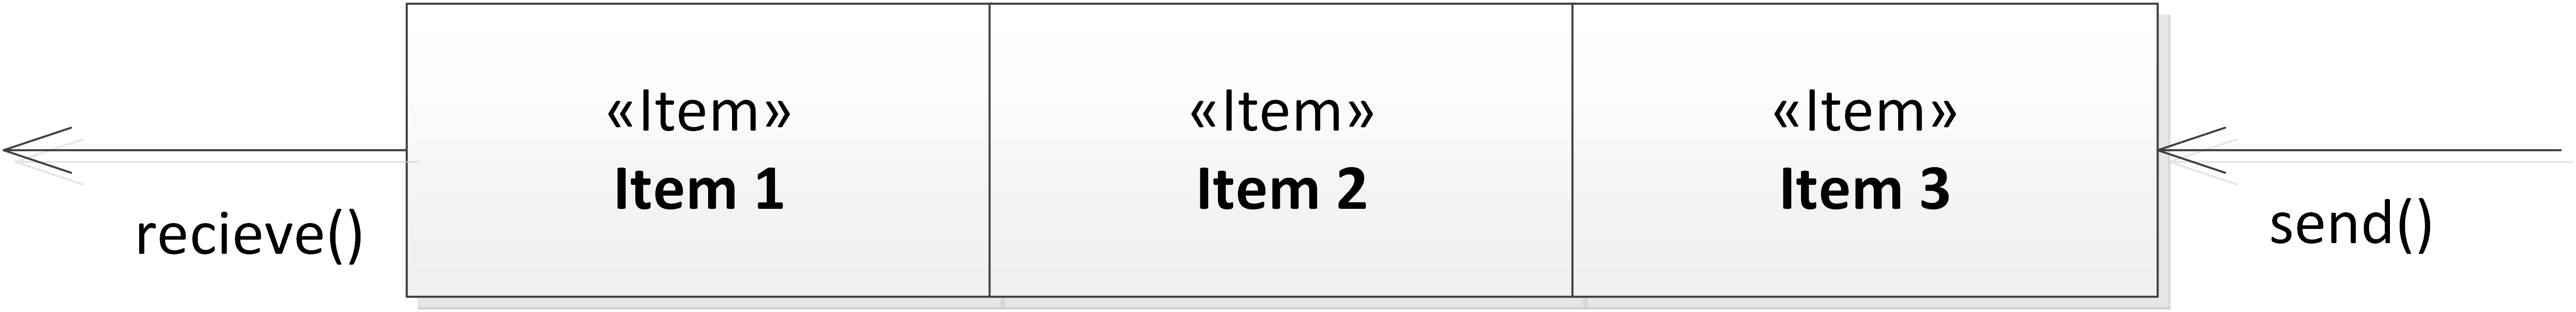
\includegraphics[scale=1]{SoftwareArkitektur/FlexPMS/Diagrammer/MessageQueue_FIFO.png}
	\caption{MessageQueue FIFO}
	\label{photo:MessageQueueFIFO}
\end{figure}


\subsubsection{Arkitekturspecifikke metoder}

\funk{void send(unsigned long id, Message* msg = NULL)}{Putter en besked i køen}{Ingenting}
{
\funkArg{id}{Event-ID som skal puttes i køen}
\funkArg{msg}{Pointer til \textit{Message}-objekt, som skal puttes i køen}
}

\funk{Message* recieve(unsigned long\& id)}{Henter den næste besked fra køen. Hvis køen er tom, så blokerer funktionen indtil der bliver puttet noget i køen via \textKode{send()}}{En pointer til et \textKode{Message}-objekt. Kan være \textKode{NULL}}
{
\funkArg{id}{Funktionen skriver event-ID til denne variabel}
}

\subsubsection{Item}

En struct, som udelukkende benyttes internt i \textit{MessageQueue}. Den holder på event ID'er og \textit{Message}-objekter, og er den type, der placeres i køen.


\subsubsection{Message}

\textit{Message} gør det muligt at medsende informationer (ud over et event-ID), når tråde kommunikerer med hinanden. Klassen \textit{Message} indeholder en \textKode{sender} attribut, som er en pointer til det \textit{MessageThread}-objekt, der sendte beskeden. \textKode{sender} gør det derfor muligt for \textit{MessageThread}'s at svare på beskeder uden at kende til afsenderen.\\\\

Alt efter hvilke data man vil sende med en besked kan man nedarve fra \textit{Message} og tilføje flere attributter.  Der er lavet specialiseringer af \textit{Message} hvor det har været nødvendigt at sende information mellem tråde.\\\\

\textbf{KarBusMessage}\\
Klassen er en specialisering af \textit{Message} og indeholder – ud over \textKode{sender} – en \textKode{kar} attribut, som er en pointer til det \textit{Kar}-objekt, der skal sendes data til. Grunden til, at \textKode{kar} kun er implementeret på \textit{KarBusMessage} er, at det altid er relevant at have information med omkring hvilket kar der skal sendes instrukser til når der kommunikeres mellem \textit{Bridge} og \textit{KarBus}, hvorimod dette ikke er nødvendigt når der kommunikeres mellem \textit{Bridge} og \textit{SocketClient}.\\
Der er adskillige specialiseringer af \textit{KarBusMessage}, som benyttes alt afhængigt af beskeden (event-ID).\\\\

\textbf{SessionMessage}\\
Klassen er en specialisering af \textit{Message} og bruges i forbindelse med, at \textit{SocketClient} skal registrere sig selv hos \textit{Bridge}. \textit{Bridge} sender en \textit{SessionMessage} til \textit{SocketClient} når klienten er registreret. Klassen indeholder en \textKode{session\_id} attribut.\\\\

\textbf{GuiMessage}\\
Klassen er en specialisering af \textit{Message} og indeholder – ud over sender – flere attributter, som bruges i forbindelse med kommunikation mellem \textit{SocketClient} og \textit{Bridge}. Klienten (webserveren) har mulighed for at sende kommandoer, som er specifikke for enten Kar eller SensorØ, og det er derfor relevant at tilføje disse attributter på \textit{GuiMessage}. Klassen indeholder desuden også en \textKode{session\_id} attribut, så Bridge ved hvilken klient den skal sende til i tilfælde, hvor svar til klienten er nødvendigt.
